\chapter{\label{ch:energyloss}Electromagnetic Energy Loss in Liquid Argon} 

%%%%%%%%%%%%%%%%%%%%%%%%%%%%%%%%%%%%%%%%%%%%%%%%%%%%%%%%%%%%%%%%%%%%%%%%%%%%%%%%
% From COS
% This chapter will cover in more detail both the theory and measurement of
% electromagnetic energy loss in liquid argon. Energy loss for both electrons and
% photons will be discussed and the implications of this for electron
% reconstruction at different energy scales will be highlighted. 
% 
% The work in this section is complete and part of this work was reported in the
% document submitted for transfer of status.
%%%%%%%%%%%%%%%%%%%%%%%%%%%%%%%%%%%%%%%%%%%%%%%%%%%%%%%%%%%%%%%%%%%%%%%%%%%%%%%%

\minitoc

The energy loss of particles in liquid argon has important implications for the
reconstruction of different particles in a LArTPC, and will be relevant for the
reconstruction algorithms developed in Chapters \ref{ch:chargeid} and 
\ref{ch:michel}. This chapter will cover in more detail the theory of 
electromagnetic energy loss in liquid argon, highlighting the important 
features of the energy loss for muons, electrons, and photons. The discussion 
here closely follows the discussion in \cite{PhysRevD.98.030001}.

\section{Electromagnetic Energy Loss in Matter}
In matter, charged particles lose energy through a number of small successive
collisions with the electrons in the material, and by radiative processes which
produce additional particles in the material. The relative importance of the
collision and radiative stopping power depends on the mass and the energy of the
particle. For most particles, which are heavy compared to the electron, 
radiative energy losses are not important until very high energies, e.g. for a 
muon they are not important until momenta of around 100 GeV, however, radiative 
energy loss become important for electrons at tens of 
MeV\cite{PhysRevD.98.030001}. As a result, different theories are used to 
describe the energy loss of heavy particles and electrons in matter.

\subsection{Energy Loss for Heavy Charged Particles}
For heavy particles, such as muons, at moderate energies, the mean rate of 
energy loss per unit distance is described by the Bethe equation,
\begin{equation}
	- \left< \frac{dE}{dx}\right> = K z^2 \frac{Z}{A} \frac{1}{\beta^2} 
	\left[ \frac{1}{2} \ln \frac{2 m_e c^2 \beta^2 \gamma^2 W_{max}}{I^2} -
	\beta^2 - \frac{\delta(\beta \gamma)}{2}\right].
	\label{eq:mu_stop}
\end{equation}
The constants in this equation are detailed in reference
\cite{PhysRevD.98.030001}. $Z$ and $A$ are the atomic number and mass number of
the medium, $z$ is the charge of the scattering particle, $W_{max}$ is the 
maximum energy transfer possible in a single collision, $I$ is the average 
ionisation energy, and $\delta$ is a density effect correction which is 
relevant in solids and liquids. 

Three important features of the energy loss in the Bethe formula are the minimum
ionising region, the relativistic rise, and the Bragg peak, these regions can be
seen in Figure \ref{fig:muon_dedx} which shows the $dE/dx$ for muons in argon 
as a function of momentum. 

\begin{figure}
	\centering
	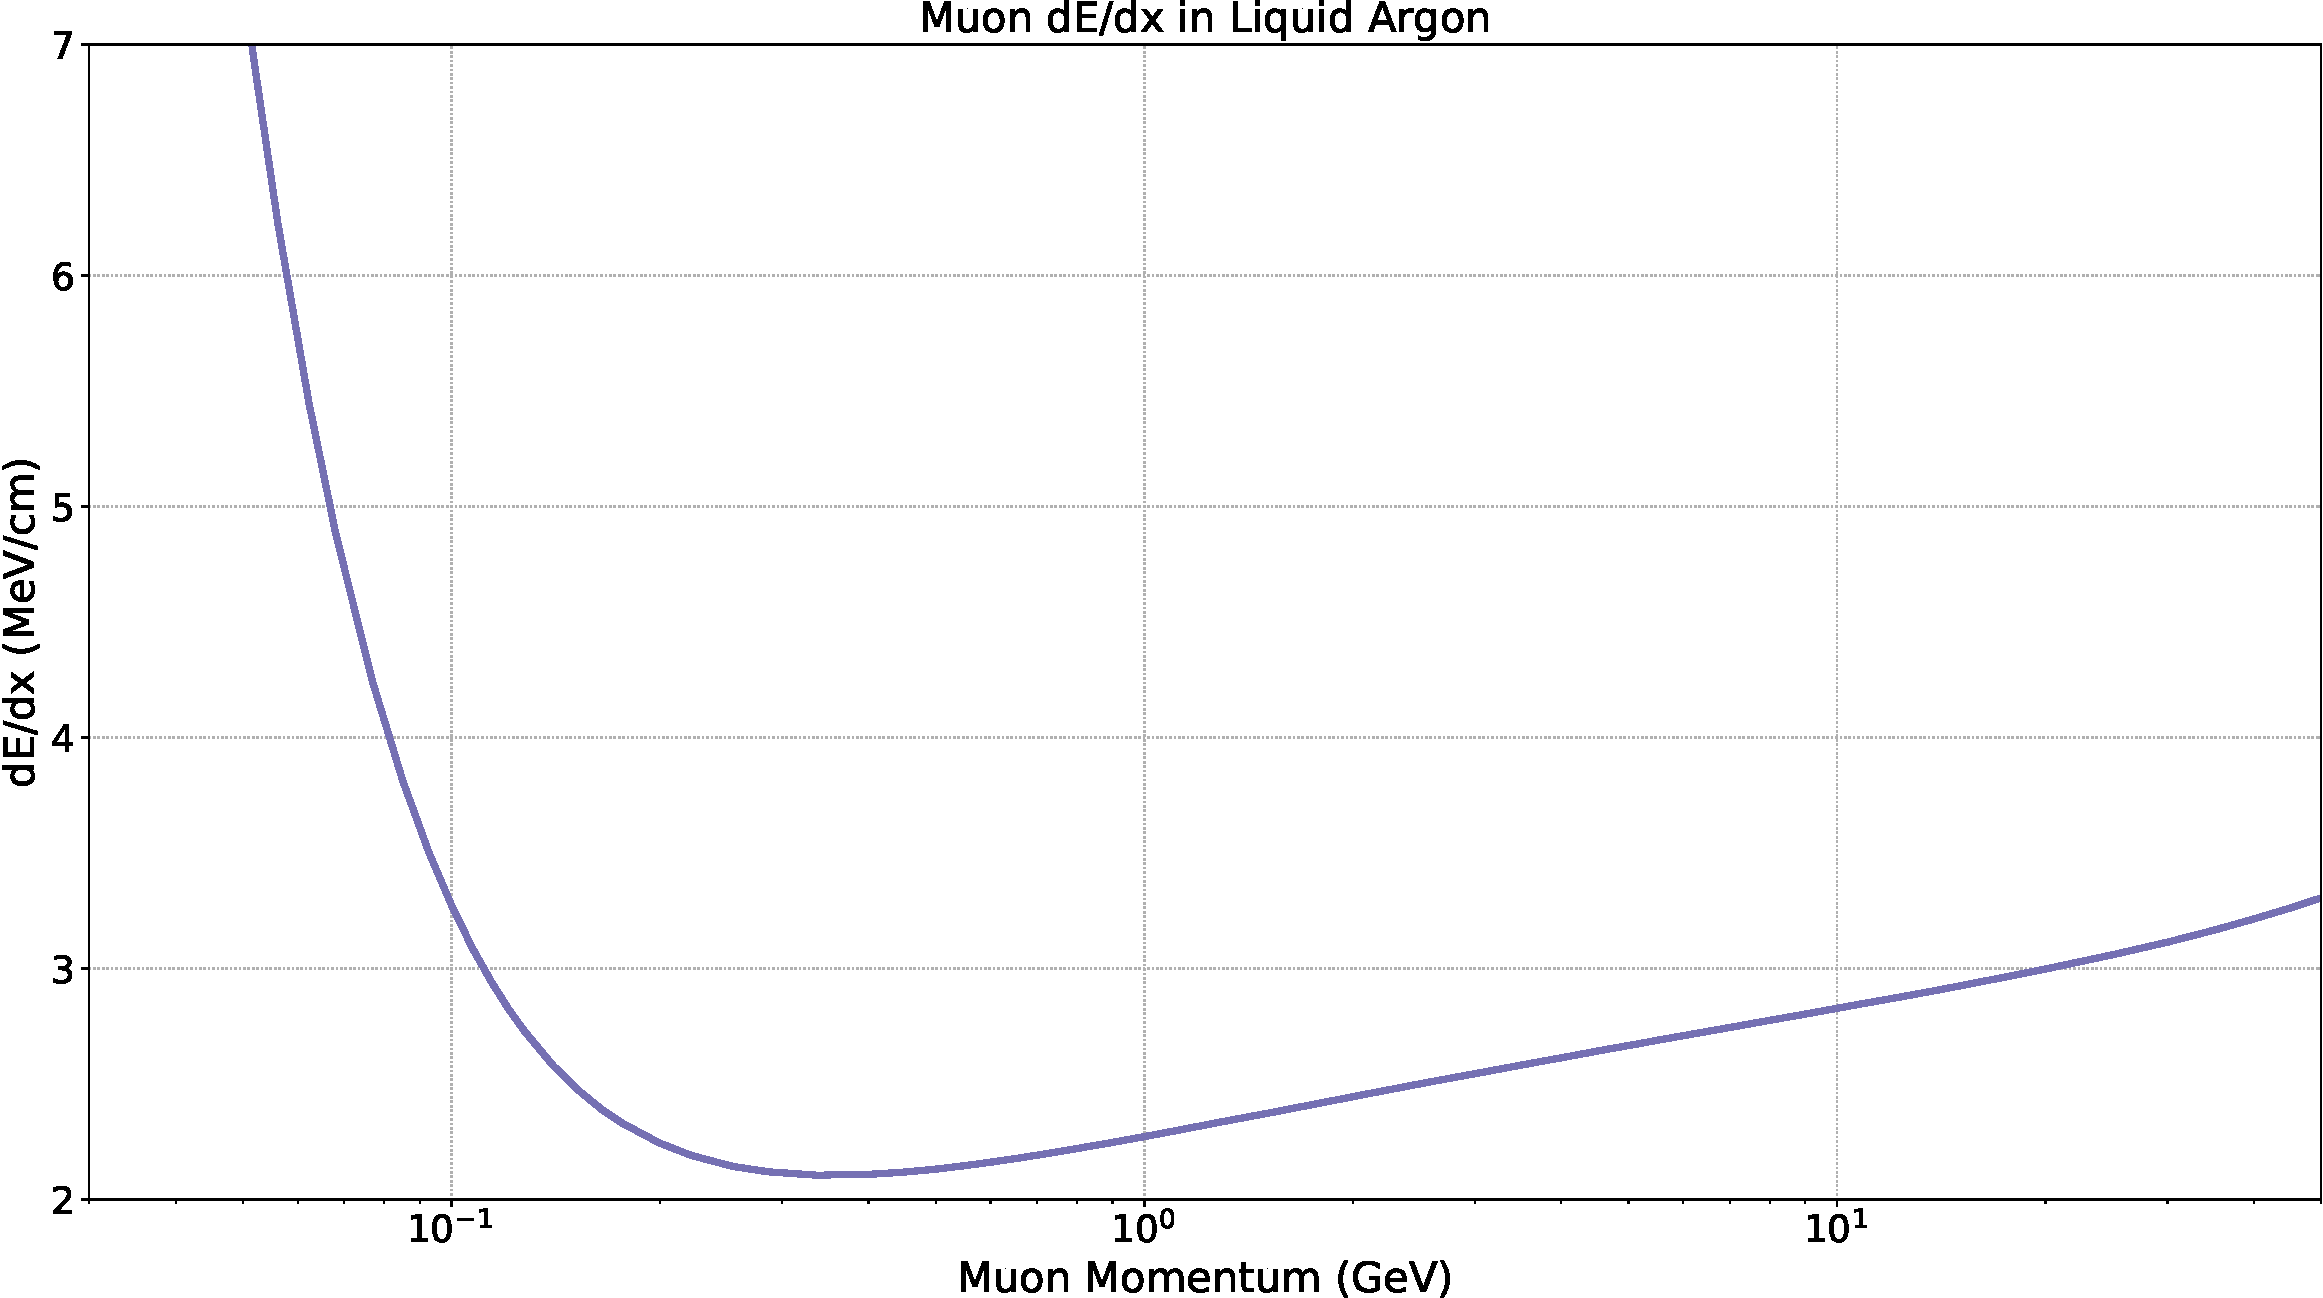
\includegraphics[width=\textwidth]{figures/muon_dedx_argon.pdf}
	\caption
	[Stopping power as a function of energy for muons in liquid argon.]
	{ Stopping power as a function of energy for muons in liquid argon. Data from
	\cite{pdg_atomictables}.}
	\label{fig:muon_dedx}
\end{figure}

\subsubsection*{Delta Rays}
Another feature of the electromagnetic energy loss of heavy particles that
impacts reconstruction in LArTPCs are delta rays. Delta rays are energetic
electrons, which are knocked out of their atom when it collides with the heavy
particle. In liquid argon detectors, these electrons are seen as small electron 
tracks which protrude from muon tracks. 

\subsection{Energy Loss for Electrons}
Electrons and positrons undergo different electromagnetic scattering processes
in matter, M{\o}ller scattering and Bhabha scattering 
respectively\cite{10.2307/96528, 10.2307/96479}. These processes, which 
dominate electron and positron energy loss at low energies, have different 
cross sections, which modify the energy loss in each case. At higher energies, 
radiative processes such as bremsstrahlung dominate. The two components of the 
electron stopping power are known as the collision stopping power and the 
radiative stopping power.

\subsubsection*{Collision Stopping Power}
The collision stopping power of electrons and positrons is calculated with a
similar method to the heavy particle stopping power, where individual collisions
are considered in succession. The main difference in the calculations is the
cross sections used in the calculations, for electrons the M{\o}ller scattering
cross section is used, and for positrons the Bhabha scattering cross section. 
Due to the electrons and positrons having the same mass as their targets, the 
maximum energy transfer in a single collision, $W_{max}$, is the total kinetic 
energy.  However, this value is halved for the case of electrons, due to the 
convention of calculating the stopping power for the final state electron with 
higher kinetic energy.

The stopping power based on M{\o}ller scattering of electrons gives,
\begin{align*}
	- \left< \frac{dE}{dx} \right> = \frac{1}{2} K \frac{Z}{A} \frac{1}{\beta^2}
	\bigg[ &\ln \frac{m_e c^2 \beta^2 \gamma^2 \left\{ m_e c^2 (\gamma - 1) / 2
	\right\} }{I^2} + (1 - \beta^2) \\
	&- \frac{2\gamma - 1}{\gamma} + \frac{1}{8} 
	\left(\frac{\gamma - 1}{\gamma}\right)^2 - \delta \bigg],
\end{align*}
while Bhabha scattering, which governs the positron stopping power, gives,
\begin{align*}
	- \left< \frac{dE}{dx} \right> = \frac{1}{2} K \frac{Z}{A} \frac{1}{\beta^2}
	\bigg[ &\ln \frac{m_e c^2 \beta^2 \gamma^2 \left\{ m_e c^2 (\gamma - 1) 
	\right\} }{2 I^2} 
	+ 2 \ln 2  \\ &-\frac{\beta^2}{12} \left(23 + \frac{14}{\gamma + 1} +
	\frac{10}{(\gamma + 1)^2} + \frac{4}{(\gamma + 1)^3}\right) - \delta \bigg],
\end{align*}
where the terms have the same meanings as in Equation 
\ref{eq:mu_stop}\cite{PhysRevD.98.030001}.

\subsubsection*{Radiative Stopping Power}
Above a few tens of MeV, electrons lose most of their energy through the 
emission of bremsstrahlung photons. Detailed discussion of the energy loss due
to bremsstrahlung emission is beyond the scope of this thesis, detailed
discussions are provided in \cite{PhysRevD.98.030001, Tsai:1973py}. A simplified
model, which highlights the important factors relevant for the work in this 
thesis, will be discussed here.

At high energies, where the radiative energy loss is dominant, the energy loss
of electrons can be approximated as energy loss over a length scale, $X_0$,  
known as the radiation length.  In this approximation, the energy loss per 
unit distance due to bremsstrahlung is, 
\begin{equation}
	- \left( \frac{dE}{dx} \right)_{brem} = \frac{E}{X_0}.
	\label{eq:rossi}
\end{equation}
The radiation length, $X_0$, can be parametrised as,
\begin{equation}
	\begin{gathered}
		\frac{1}{X_0} = 4 \alpha r_e^2 \frac{N_A}{A} \left\{ Z^2 \left[L_{rad} - f(Z)\right] + Z
		L^\prime_{rad} \right\} \\
		\begin{aligned}
			f(Z) = \alpha^2 Z^2 \bigg[ &\frac{1}{1 + \alpha^2 Z^2} + 0.20206 - 0.0369
			\alpha^2 Z^2 \\ &+ 0.0083 \alpha^4 Z^4 -0.0002 \alpha^6 Z^6 \bigg],
		\end{aligned}
	\end{gathered}
	\label{eq:rad_length}
\end{equation}
where $L_{rad}$ and $L_{rad}^\prime$ are the so--called radiation logarithms,
which depend on the atomic number of the material\cite{Tsai:1973py}.

\subsubsection*{Critical Energy}
Critical energy is often defined as the energy at which the collision and 
radiative stopping power are equivalent, other definitions are also used, such
as the definition by Rossi, the energy where the ionisation loss per
radiation length is equal to the electron energy\cite{Rossi:1952kt}. Rossi's 
definition is equivalent to using the approximate $dE/dx$ in Equation 
\ref{eq:rossi}\cite{PhysRevD.98.030001}. The value of the critical energy has 
important implications for reconstruction algorithms, because different 
approaches are often required above and below the critical energy. 

The critical energy is slightly different for electrons and positrons, in 
liquid argon they are both around 32 MeV, based on the Rossi 
definition\cite{pdg_atomictables}. This can be seen in Figure 
\ref{fig:electron_dedx}, which shows the total electron stopping power in 
liquid argon, in addition to the collision and radiative components which make 
up the total stopping power. 

\begin{figure}

	\centering

	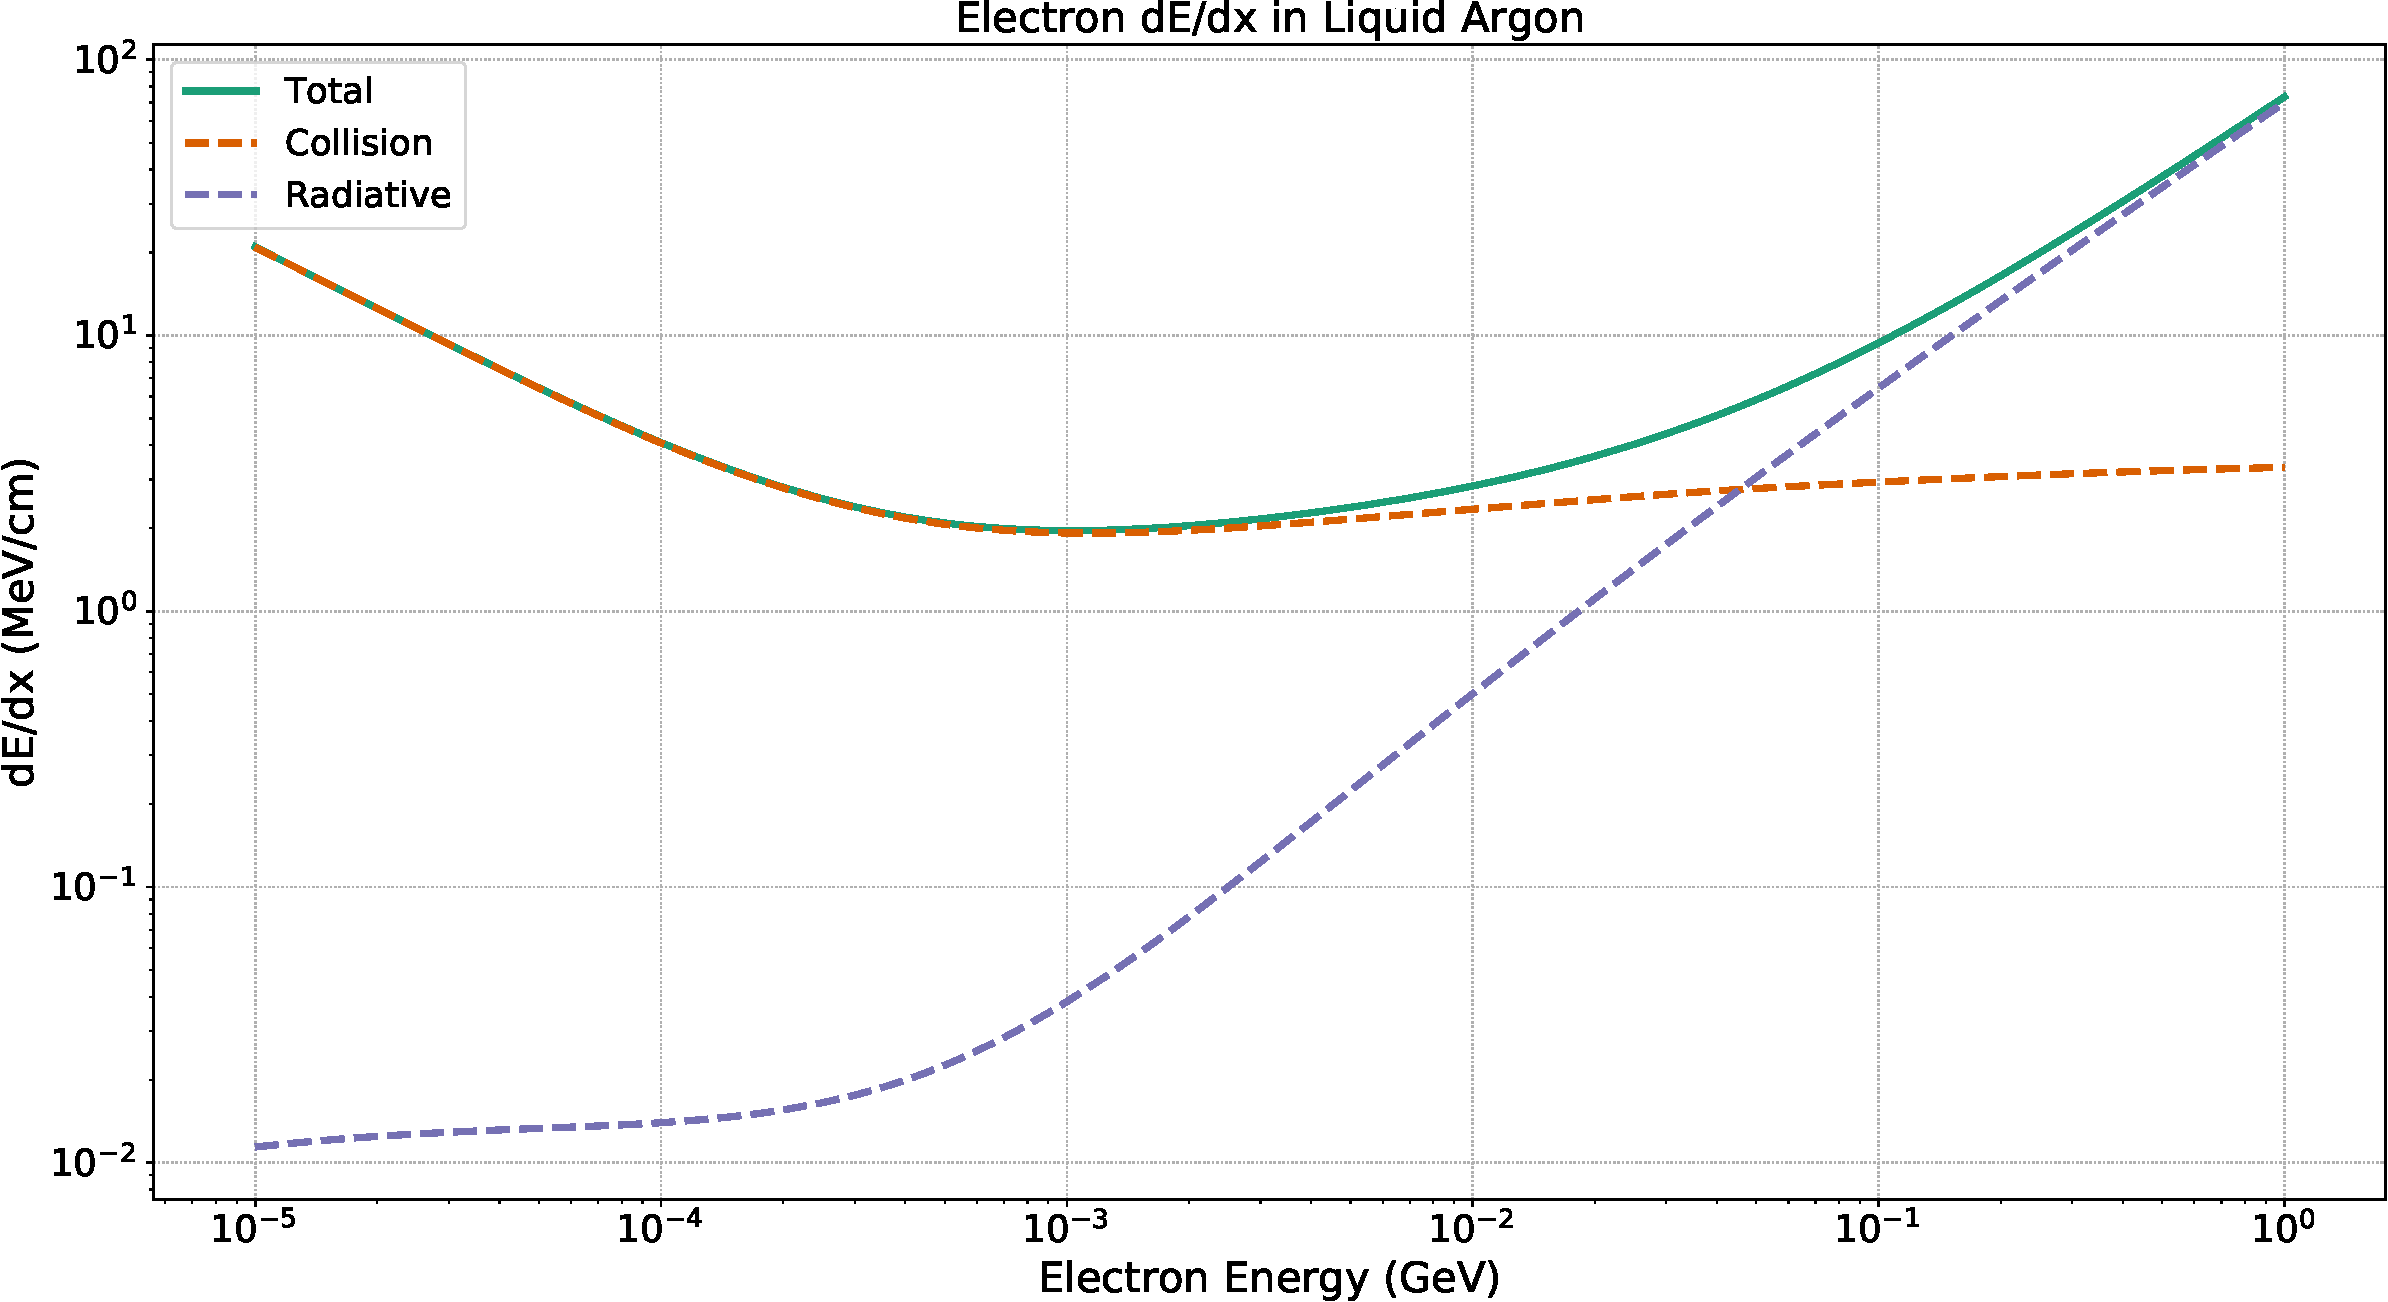
\includegraphics[width=\textwidth]{figures/electron_dedx_argon.pdf}

	\caption
	[Stopping power as a function of energy for electrons in liquid argon.]
	{Stopping power as a function of energy for electrons in liquid argon. The
	contributions from collision and radiative stopping power are shown as dashed
	lines. The total stopping power is shown as a solid line. Data from 
	\cite{estar}.}

	\label{fig:electron_dedx}

\end{figure}

\subsection{Energy Loss for Photons}
A number of processes contribute to the energy loss of photons in matter, brief 
descriptions of the main processes are given below.

\subsubsection*{Photoelectric Effect}
The photoelectric effect occurs when a photon collides with an atom, X, the
photon is absorbed and electron is emitted from the atom. As a result, the atom 
is ionised. 
\begin{equation*}
	\gamma + X \rightarrow e^- + X^+
\end{equation*}

\subsubsection*{Compton Scattering}
Compton scattering occurs when a photon scatters incoherently from an electron
within an atom. The electron is typically liberated from the atom, and the
photon loses some of it's energy.
\begin{equation*}
	\gamma + e^- \rightarrow \gamma + e^-
\end{equation*}

\subsubsection*{Pair Production}
Pair production is the production of an electron positron pair, in the 
vicinity of an external electric field. During this process, the photon is
destroyed to produce the electron positron pair. In matter, the electric field
could be provided by either the electrons in the atom, or the nucleus of the
atom.
\begin{equation*}
	\gamma \rightarrow e^+ + e^-
\end{equation*}

\medskip\noindent
The cross section for these effects vary as a function of photon energy. The 
cross sections for each process in liquid argon, as well as the total photon 
cross section, are given in Figure \ref{fig:photon_xsec}. The Compton scattering
cross section is dominant from around 0.1 MeV to 10 MeV, after which the pair
production cross section dominates. 

\begin{figure}

	\centering

	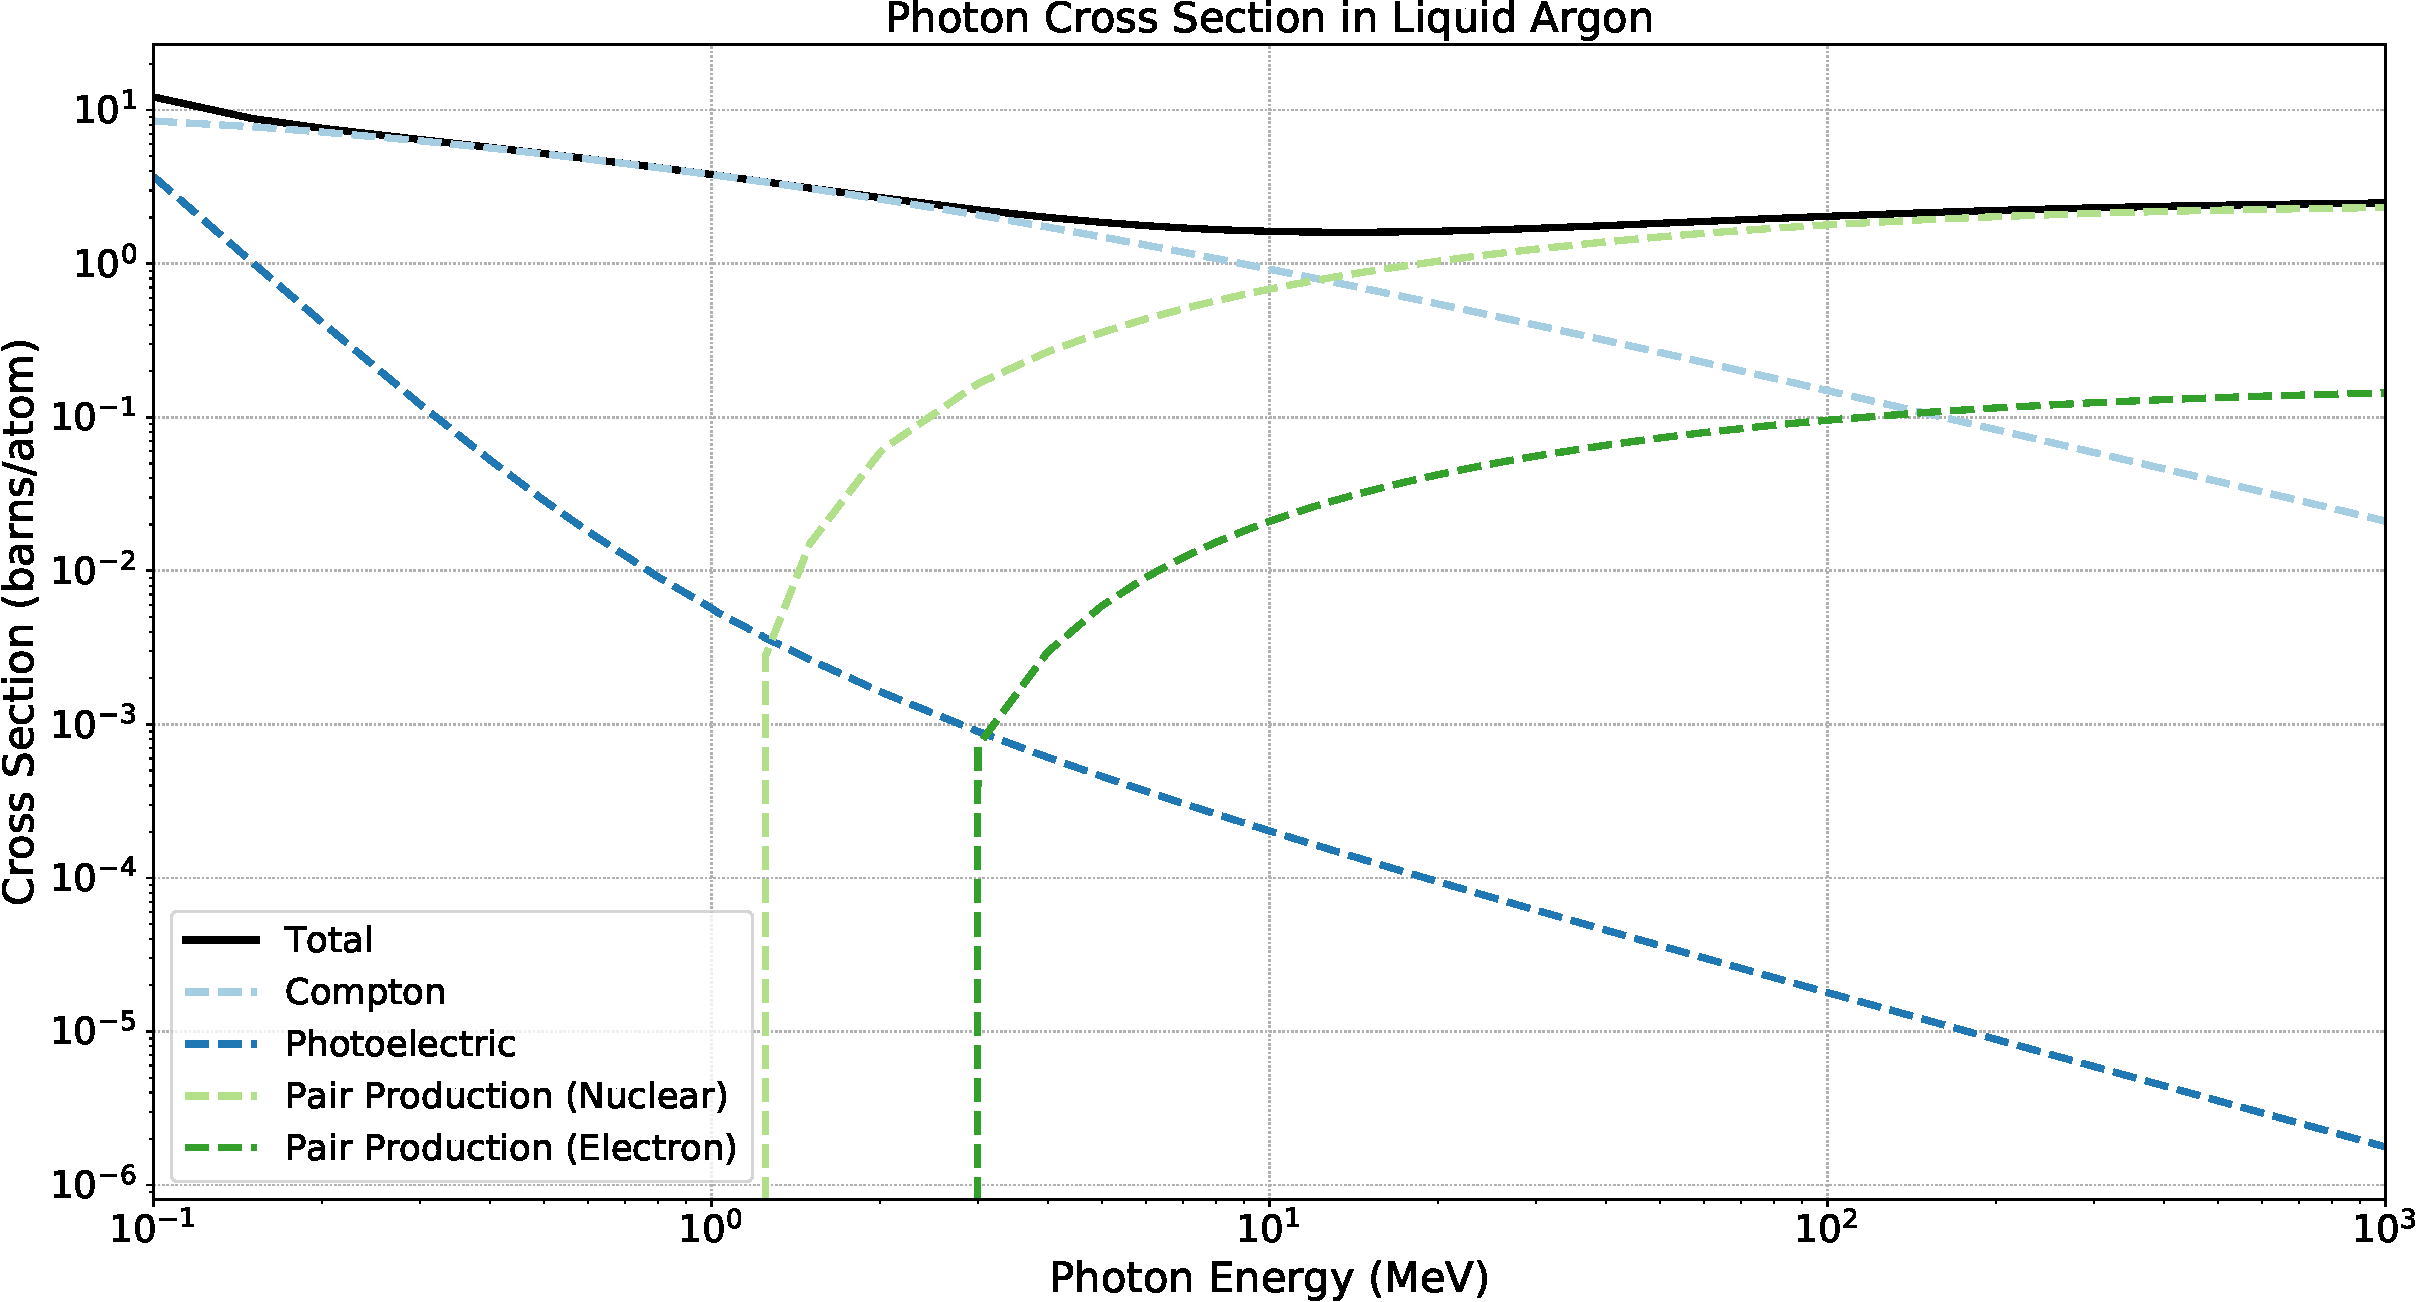
\includegraphics[width=\textwidth]{figures/photon_xsec.pdf}

	\caption
	[Photon interaction cross sections in liquid argon.]
	{ Photon interaction cross sections in liquid argon. The contributions from
	Compton scattering, photo--electric effect, and pair production are shown as
	dashed lines. The total photon cross section is shown as a solid line. Data 
	from \cite{photon_xsection}.}

	\label{fig:photon_xsec}

\end{figure}

\subsubsection*{Photon Mean Free Path}
The mean free path of a photon is defined as the average distance travelled by 
the photon before it interacts with the material. The mean free path for 
photons has two main components for photons in the MeV range, which are 
Compton scattering and pair production. The mean free path is given by 
$\lambda = 1 / (n \sigma)$, where $n$ is the number density of targets and 
$\sigma$ is the cross section per target. The contribution to the mean free 
path from pair production is related to the radiation length for electrons, 
$X_0$ from Equation \ref{eq:rad_length}, by $\lambda_{PP} = (9/7) \; 
X_0$\cite{PhysRevD.98.030001}.  The mean free path for photons in the MeV 
range is shown in Figure \ref{fig:photon_mfp}, along with the main 
contributing cross sections. 

\begin{figure}

	\centering

	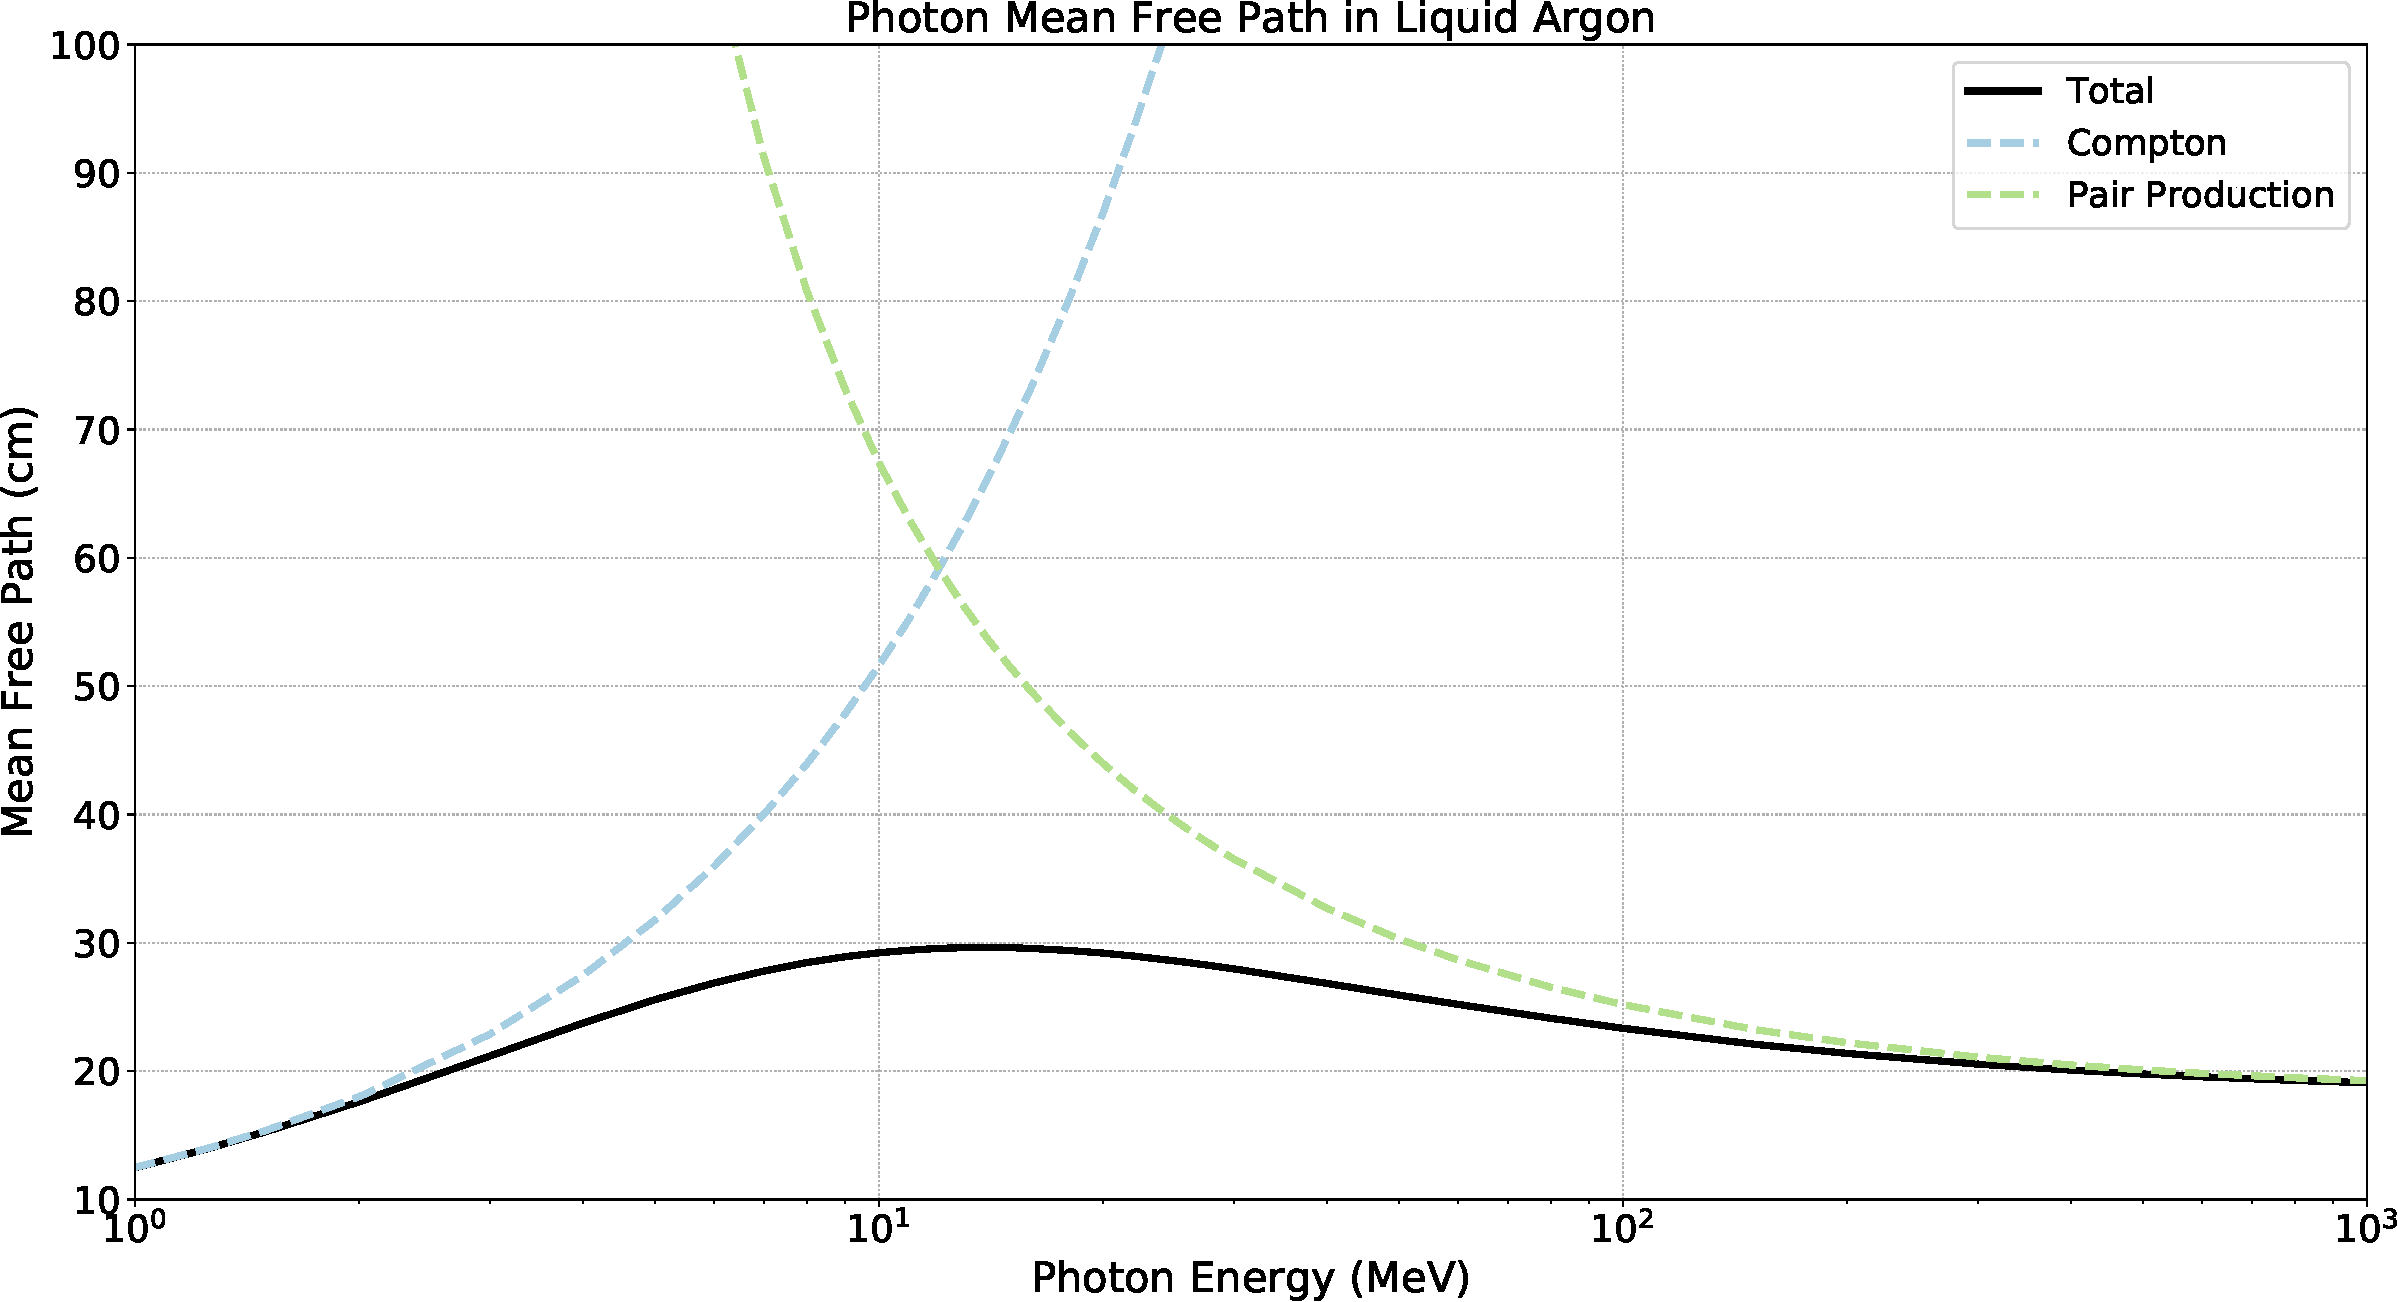
\includegraphics[width=\textwidth]{figures/photon_mfp.pdf}

	\caption
	[Photon mean free path in liquid argon.]
	{Photon mean free path in liquid argon. The mean free path based on the cross
	sections for Compton scattering, photo--electric effect, and pair production 
	are shown as dashed lines. The total photon mean free path is shown as a 
	solid line. Data from \cite{photon_xsection}.}

	\label{fig:photon_mfp}

\end{figure}

\section{Interaction Signatures in \protodune{}}
As a result of the differences in energy loss, which depend on particle species
and energy, different particles leave distinct signatures in the detector.  
Figure \ref{fig:particle_signatures} shows the typical signatures of four 
types of interaction in a liquid argon TPC, for events from \protodune{} 
data.

\begin{figure}

	\centering

	\begin{subfigure}[b]{0.49\textwidth}
		\centering
		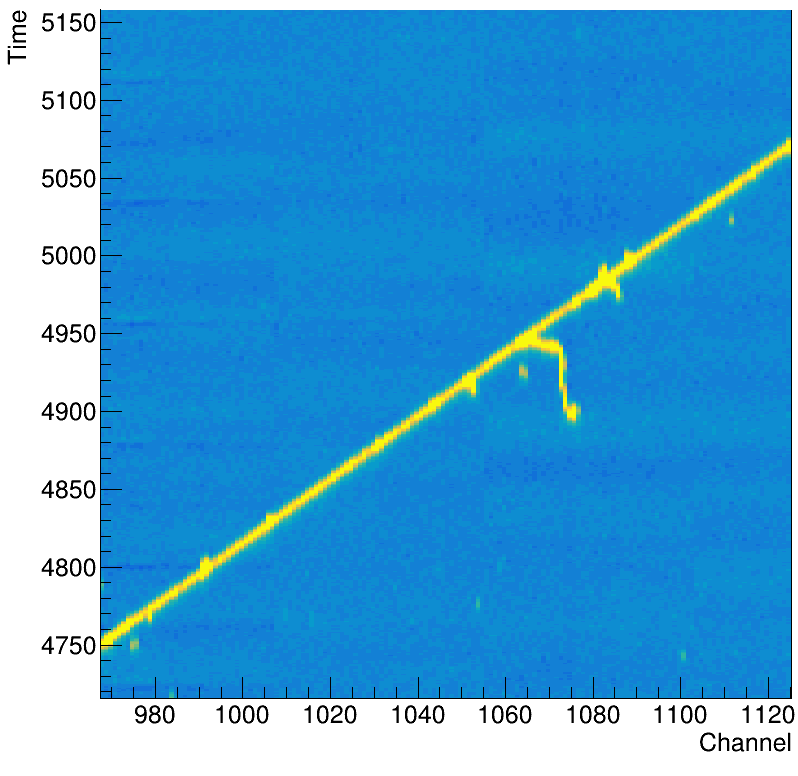
\includegraphics[width=\textwidth]{figures/muon_signature.png}
		\caption{Muon track with delta rays.}
		\label{fig:muon_signature}
	\end{subfigure}
	\hfill
	\begin{subfigure}[b]{0.49\textwidth}
		\centering
		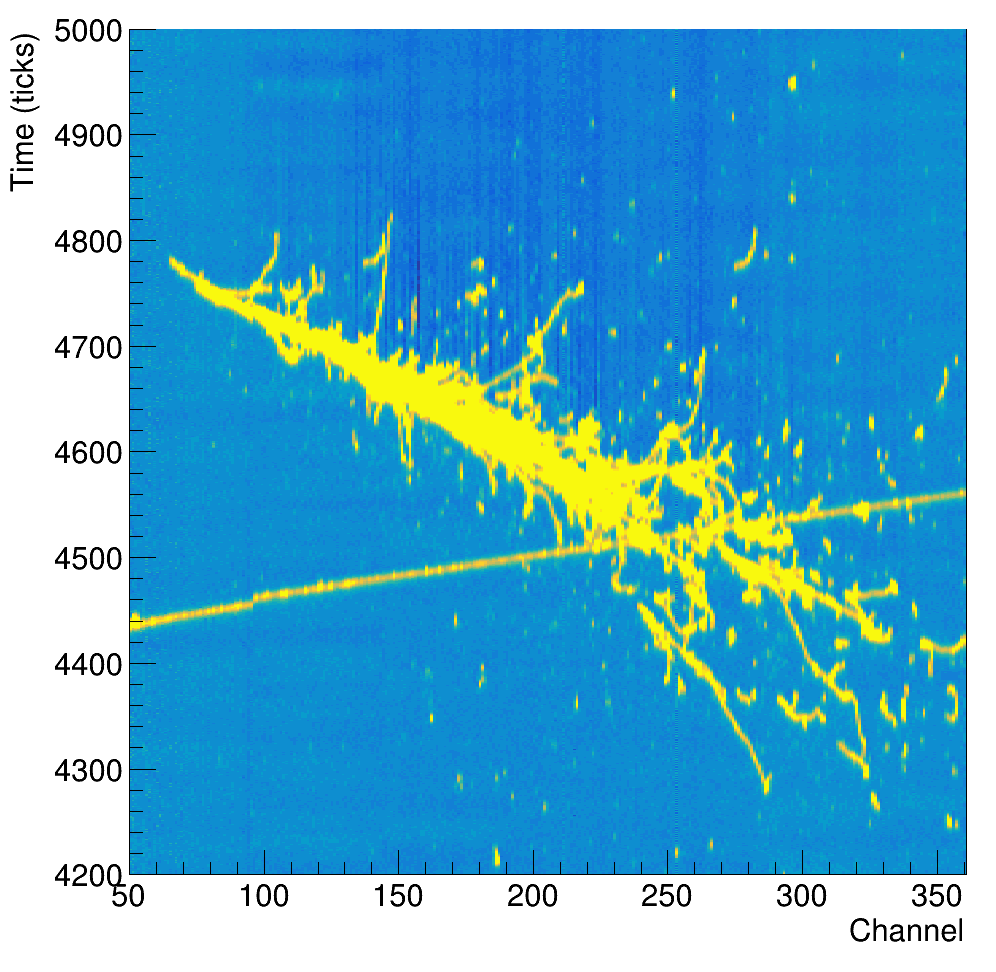
\includegraphics[width=\textwidth]{figures/electron_signature.png}
		\caption{Electron shower.}
		\label{fig:electron_signature}
	\end{subfigure}

	\begin{subfigure}[b]{0.49\textwidth}
		\vspace{5mm}
		\centering
		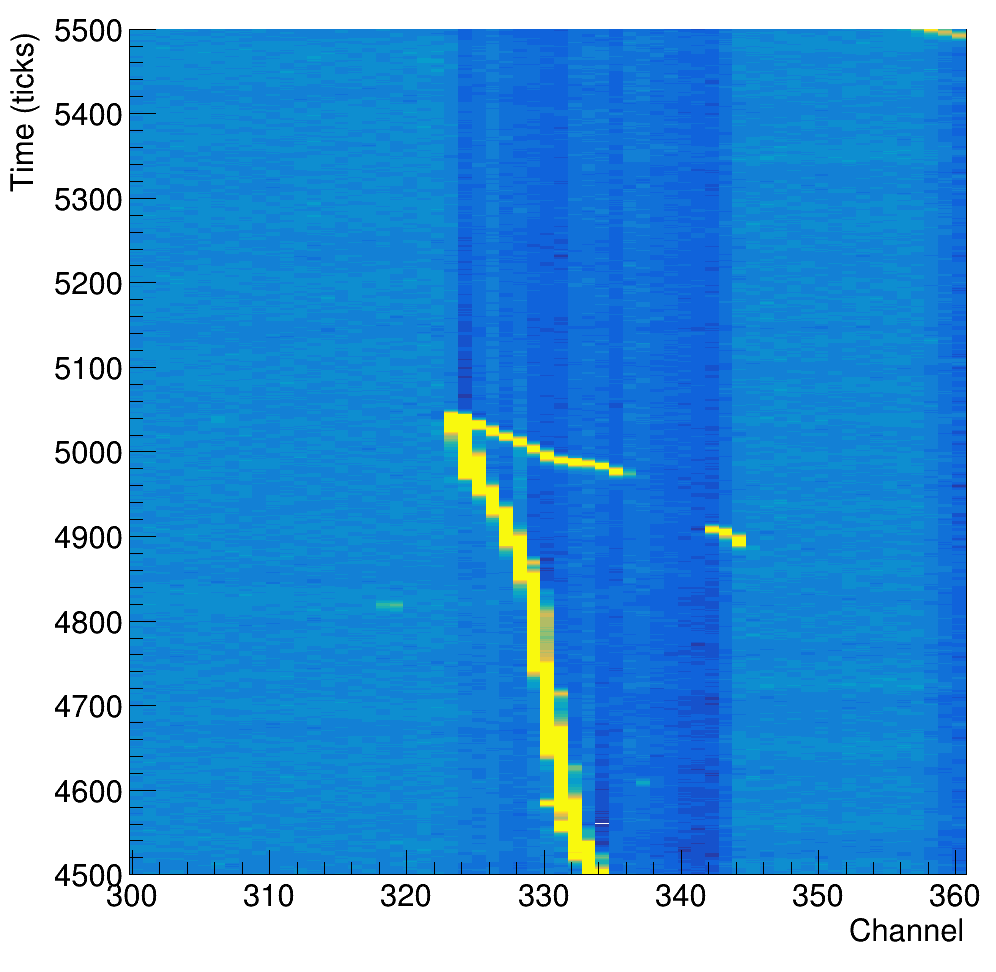
\includegraphics[width=\textwidth]{figures/michel_signature.png}
		\caption{Michel electron.}
		\label{fig:michel_signature}
	\end{subfigure}
	\hfill
	\begin{subfigure}[b]{0.49\textwidth}
		\vspace{5mm}
		\centering
		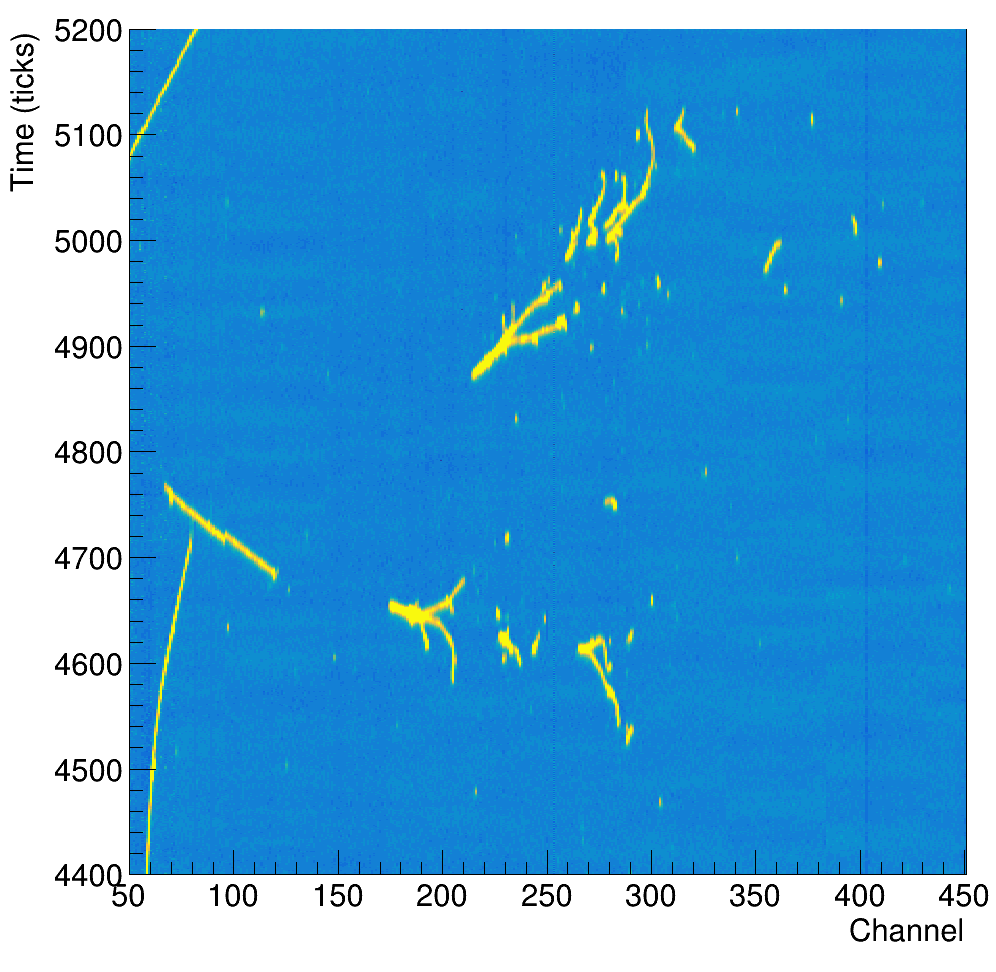
\includegraphics[width=\textwidth]{figures/pi0_signature.png}
		\caption{Photon showers from a $\pi^0$ decay.}
		\label{fig:pi0_signature}
	\end{subfigure}

	\caption
	[Typical particle signatures in \protodune{} for different particle 
	species.]
	{Typical particle signatures in \protodune{} data for candidate particles
	from different particle species. These images are made from the raw detector
	readout on the collection plane, before noise filtering and deconvolution are 
	applied. }

	\label{fig:particle_signatures}

\end{figure}

The most common interaction in \protodune{} is that of a cosmic--ray muon, seen
in Figure \ref{fig:muon_signature}. Muons, and other heavy particles, leave 
long tracks in the detector which deposit around 2.1 MeV/cm in the minimum 
ionising region. Alongside muon tracks, relatively high energy electrons, 
known as delta rays, are occasionally produced. Delta rays can be seen as 
electron activity along the length of the muon track.

Electrons in \protodune{} have two distinct signatures, which depend on the
energy of the electron. For high energy electrons, with energies above around
300 MeV, radiative energy loss dominates and showers are produced, an example 
of an electron shower can be seen in Figure \ref{fig:electron_signature}. 
These showers are the result of a cascade of electrons, which are produced by 
a chain of bremsstrahlung photons and electron positron pairs. At energies in 
the tens of MeV range electrons have a different signature, which consists of 
a small electron track accompanied by a number of small ionisation energy 
deposits due to radiated photons. 

A common source of tens of MeV electrons in \protodune{} are Michel electrons, 
which are the electrons produced when a muon decays at rest in the detector. 
An example of a typical Michel electron event is shown in Figure 
\ref{fig:michel_signature}. The Michel electron is accompanied by the incoming 
Muon in the image, because the lifetime of the muon is shorter than the time 
it takes for the ionisation charge to drift away from the stationary muon.

As with electrons, photon interactions in liquid argon have two distinct
signatures at high and low energies. Low energy photons are typically produced
by the interactions of low energy electrons in the liquid argon, such as the
Michel electron interaction in Figure \ref{fig:michel_signature}. When these 
photons interact they produce small isolated energy deposits, which are 
created by the ionisation from either Compton scattered electron or an electron 
positron pair.

At high energies, photons produce similar interactions to high energy electrons,
which produce electromagnetic showers in the liquid argon. There is a slight
difference in the $dE/dx$ in the first few cm of electron and photon showers, 
because the start of photon showers contain two electrons whereas the start of
electron showers only have one. This difference can allow for electron and 
photon showers to be distinguished from each other\cite{Acciarri:2016sli}. A 
common source of photon showers in \protodune{} are $\pi^0$ decays, shown in 
Figure \ref{fig:pi0_signature}, which produce a pair of photons.

\section{Scintillation Light in Liquid Argon}
The second source of electromagnetic energy loss in liquid argon is due to the
production of scintillation light. As the work in this thesis does not make
use of the scintillation energy depositions, the mechanisms involved in the 
production of scintillation light will only be briefly summarised here for 
completeness.

Scintillation light in liquid argon is produced by radiative decay of excited
argon dimers (or eximers), which are produced when excited argon atoms combine
with a ground state argon atom to form an excited $\mbox{Ar}_2$ molecule. Two 
excited dimer states contribute to the scintillation light production, a 
singlet and a triplet, with lifetimes of $6 \mbox{ ns}$ and $1.5 \mbox{ } \mu 
\mbox{s}$ respectively\cite{Lippincott:2008ad}. When the dimers decay they 
produce two ground state argon atoms, and release scintillation light 
isotropically in the form of $128 \mbox{ nm}$ photons. Argon is transparent to 
these photons and, therefore, the scintillation light can travel large 
distances before being collected by a photon detection system.
